\documentclass{article}
\usepackage{amsmath}
\usepackage{listings}
\usepackage{hyperref}
\usepackage{geometry}
\usepackage{graphicx}
\usepackage{amssymb}
\usepackage{array}

% Page settings
\geometry{a4paper, margin=1in}

% Title Information
\title{Architecture COMP15111 Course Notes}
\author{Molshin Nurassyl}
\date{}

\begin{document}

\maketitle

\tableofcontents

% Week 1 Notes
\newpage
\section*{Week 1: Introduction to Computer Architecture}
\addcontentsline{toc}{section}{Week 1: Introduction to Computer Architecture}

\subsection*{Introduction}
\begin{itemize}
    \item How components of a computer fit together to execute programs.
    \item The hardware programming model.
    \item Microarchitecture.
    \item System architecture.
\end{itemize}

\subsection*{Computer Architecture and Hardware Design}
\textbf{Bus:} How the resources are organized
\begin{itemize}
    \item How it is actually implemented.
\end{itemize}

\textbf{RISC-V and ARM}
\begin{itemize}
    \item Can be implemented in different processors.
    \item Can run programmable hardware (FPGA).
    \item Can run in software (simulated).
\end{itemize}

\subsection*{Computer Architecture}
Computer architecture cares about the high-level design and organization of the processor. It connects hardware and software together.

\subsection*{What is a Program?}
\begin{itemize}
    \item Apps, OS, Online Services, AI models.
    \item A sequence of unambiguously specified computer operations that collectively achieve a purpose.
\end{itemize}

\subsection*{How Does This Work?}
\begin{align*}
    \text{Users write} &\rightarrow \text{ High Level Programs} \\
    \text{Compiled into} &\rightarrow \text{ Assembly} \\
    \text{Assembled into} &\rightarrow \text{ Machine Code} \\
    \text{Which is executed} &\rightarrow \text{ Hardware}
\end{align*}

\subsection*{Levels of Abstraction}
\begin{enumerate}
    \item \textbf{Higher Levels (Human)}
    \begin{itemize}
        \item Easier to understand.
        \item Can run on different systems.
        \item Less control.
    \end{itemize}

    \item \textbf{Lower Levels (Machine Code)}
    \begin{itemize}
        \item Precise control.
        \item Specific for each computer family.
    \end{itemize}

    \item \textbf{Assembly Language (Compromise)}
    \begin{itemize}
        \item Uses RISC-V.
    \end{itemize}
\end{enumerate}

\subsection*{Registers}
\begin{itemize}
    \item Memory inside the CPU.
    \item Limited size but super fast.
\end{itemize}

\subsection*{Load-Store Architecture}
\begin{itemize}
    \item Operation operands are registers.
    \item Load instructions read data from memory into a register.
    \item Store instructions write data from a register into memory.
    \item More efficient use of memory.
    \item Simpler and faster instructions.
\end{itemize}

\subsection*{RISC-V}
\begin{itemize}
    \item 32 registers.
    \item 32-bit wide.
    \item \( x0 \) to \( x31 \).
\end{itemize}

\subsection*{The RISC-V Instruction Set}
\begin{figure}
    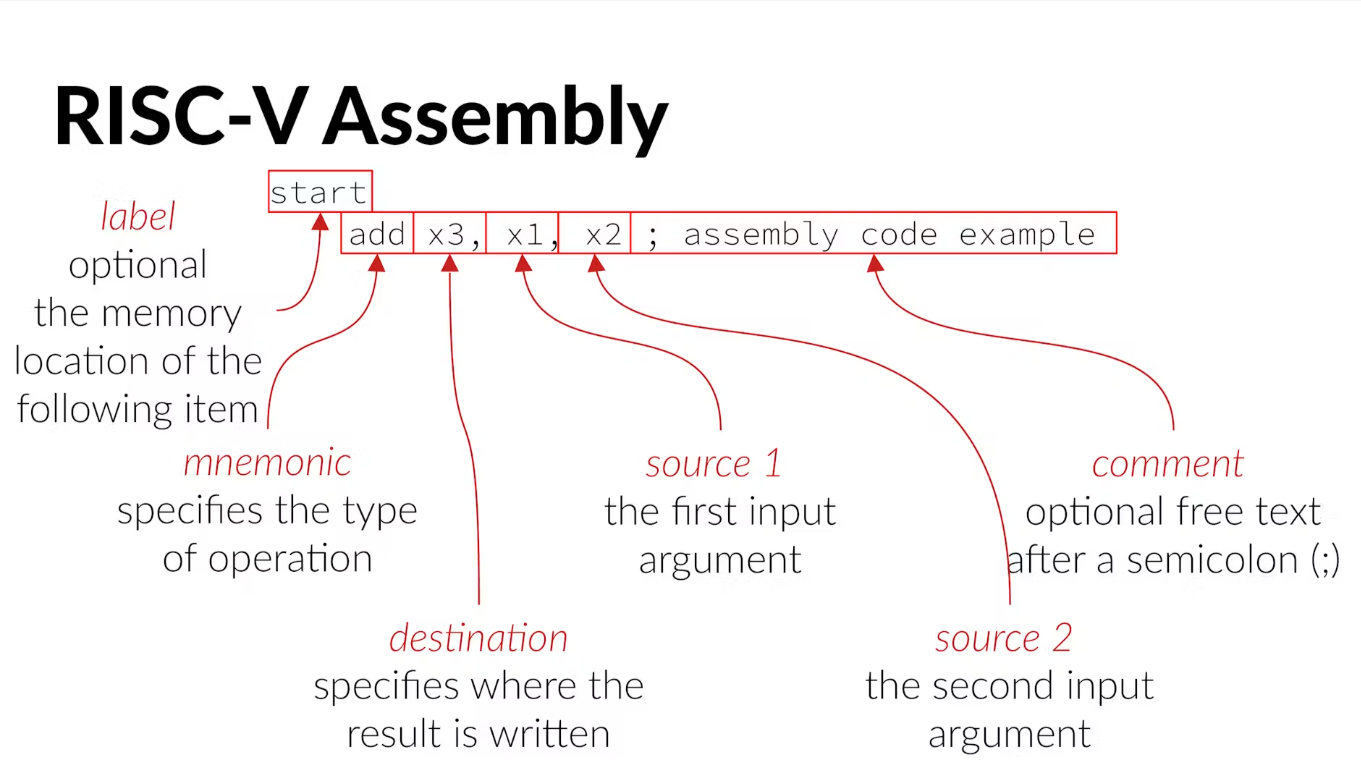
\includegraphics[width=15cm]{images/Instructionconstruction.png}
    \caption{How instruction looks like}
    \label{figure:instruction}
\end{figure}
    

\subsection*{Data Processing Instructions}
\begin{itemize}
    \item Arithmetic, Logic, Shift, or Comparison.
    \item General format:
\end{itemize}
\begin{lstlisting}
mnemonic rd, rs1, rs2 ; or
mnemonic rd, rs1, imm;
\end{lstlisting}

\subsection*{Instruction Types}
\begin{figure}
    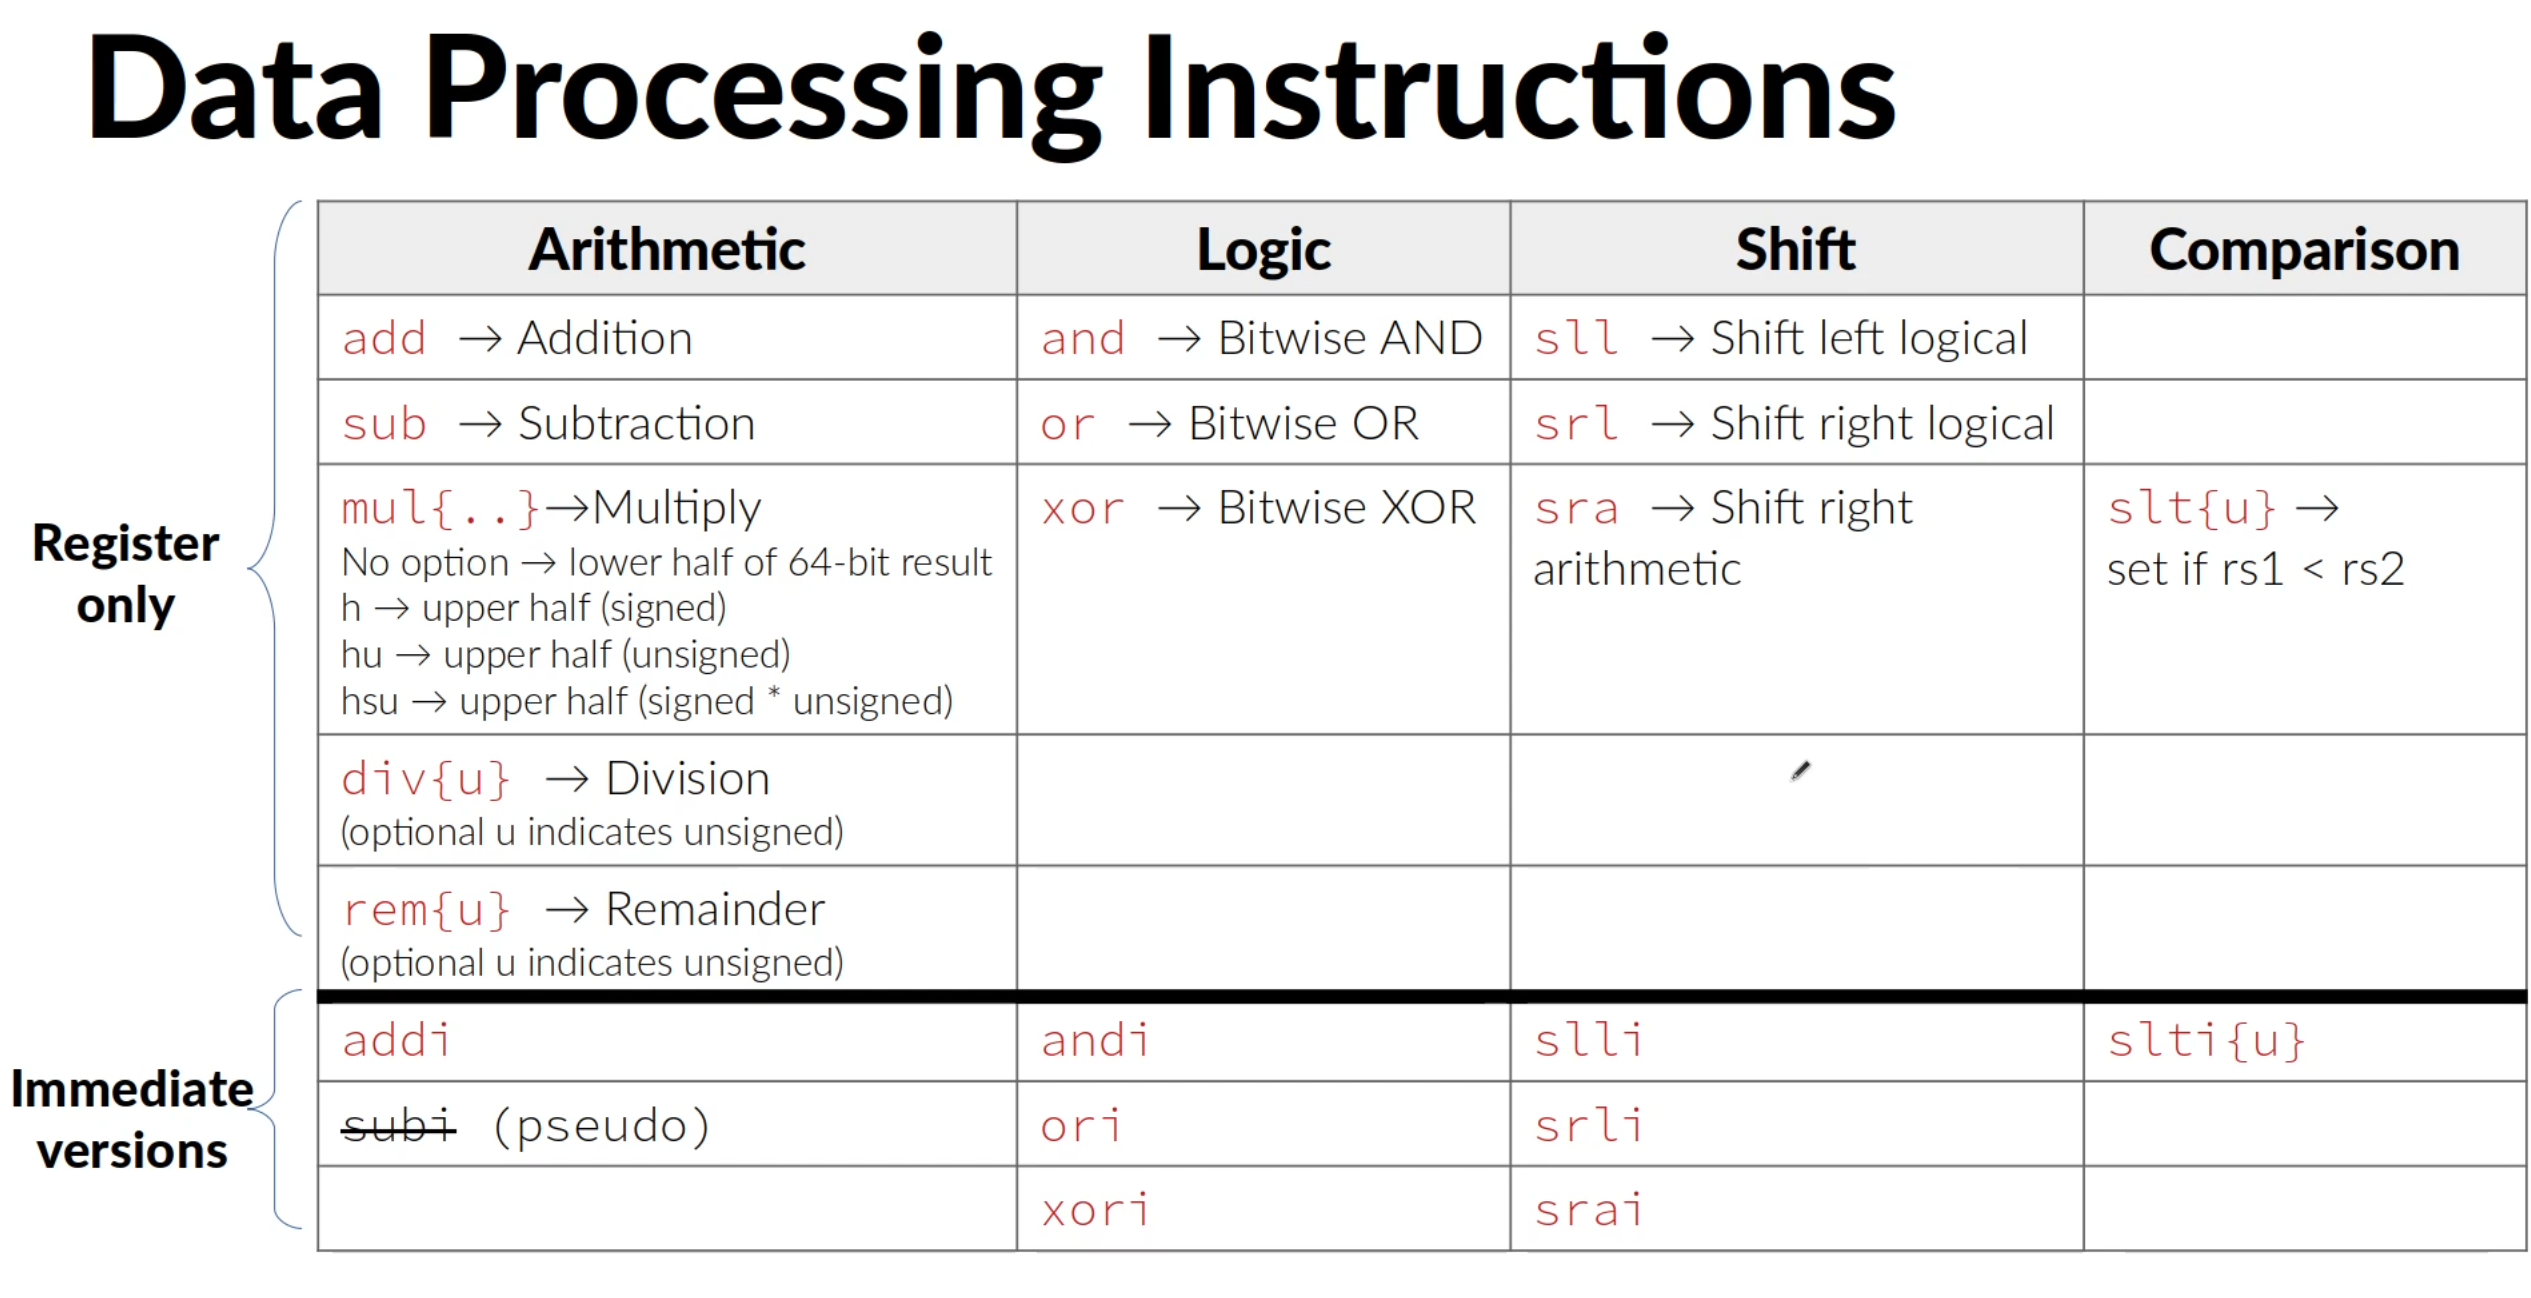
\includegraphics[width=15cm]{images/dtprcsinstrc.png}
    \caption{Data Processing instructions}
    \label{figure:dtprcsinstrc}
\end{figure}

\subsubsection*{Comparison}
\begin{align*}
    \text{slt} \{x, y\} &\rightarrow \text{Set if rs1 < rs2}
\end{align*}

\subsection*{Memory Operations}
\begin{itemize}
    \item Load: \texttt{lw rd, imm(rs)}
    \item Store: \texttt{sw rs2, imm(rs1)}
\end{itemize}

\begin{lstlisting}
sum = a + b + c
lw x1, a
lw x2, b
add x3, x1, x2
\end{lstlisting}

\subsection*{Example Program}
\begin{lstlisting}
lw x3, c
add x4, x3, x2 ; (a + b) + c
sw x5, sum, x6
\end{lstlisting}




\newpage
\section*{Week 2: Control Flow and Representation of Information}
\addcontentsline{toc}{section}{Week 2: Control Flow and Representation of Information}


\section*{Control Flow}
\textbf{The Fetch Execute Cycle:}
\begin{itemize}
    \item \textbf{Initialisation} (PC contains the address of the first instruction, normally 0)
    \item \textbf{Fetch}
    \begin{itemize}
        \item Read the word in the location pointed to by PC
        \item Increment PC by 4
    \end{itemize}
    \item \textbf{Execute}
    \begin{itemize}
        \item Decode the instruction
        \item Apply the operation on operands
        \item Repeat forever
    \end{itemize}
    \item \textbf{Execution is serial} (Going down the list of instructions)
    \item \textbf{Little flexibility}
    \begin{itemize}
        \item Cannot reuse instructions without copy-pasting
        \item Cannot change what is executed
    \end{itemize}
\end{itemize}

\section*{Flow Control Instructions}
\textbf{Jump} - Unconditional flow instructions \\
\textbf{Branch} - Conditional flow instructions

\subsection*{Unconditional Control Flow}
\begin{itemize}
    \item \texttt{jal rd, label}
    \begin{itemize}
        \item Jump and Link
        \item Next instruction stored in \texttt{rd}: \quad \texttt{rd} $\leftarrow$ \texttt{PC+4}
        \item Execution jumps to the address represented by \texttt{label}: \quad \texttt{PC} $\leftarrow$ \texttt{label}
    \end{itemize}
    \item \texttt{jalr rd, rs1, imm}
    \begin{itemize}
        \item Jump and Link with register
        \item Next instruction stored in \texttt{rd}: \quad \texttt{rd} $\leftarrow$ \texttt{PC+4}
        \item Execution jumps to the address represented by \texttt{rs1 + imm}: \quad \texttt{PC} $\leftarrow$ \texttt{rs1 + imm}
    \end{itemize}
\end{itemize}

\subsection*{Conditional Control Flow}
\textbf{General Syntax}
\begin{itemize}
    \item \texttt{beq cond, rs1, rs2, label}
    \item Branch if \texttt{cond}
    \item If \texttt{cond} is true for \texttt{rs1} and \texttt{rs2}: \quad \texttt{PC} $\leftarrow$ \texttt{label}
    \item If \texttt{cond} is false: \quad \texttt{PC} $\leftarrow$ \texttt{PC+4}
\end{itemize}

\textbf{Conditions:}
\begin{itemize}
    \item \texttt{eq} = equal
    \item \texttt{ne} $\neq$ not equal
    \item \texttt{lt\{u\}} $<$ less than
    \item \texttt{le\{u\}} $\leq$ less or equal
    \item \texttt{gt\{u\}} $>$ greater
    \item \texttt{ge\{u\}} $\geq$ greater or equal
\end{itemize}

\textbf{Branch Pseudo-Instructions:}
\begin{itemize}
    \item \texttt{blt} and \texttt{bgt} are symmetrical
    \item \texttt{blt x1, x2, target} $\Rightarrow$ \texttt{x1 < x2} \quad \texttt{bgt x2, x1, target} $\Rightarrow$ \texttt{x1 > x2}
\end{itemize}

\subsection*{Test for Zero}
\begin{itemize}
    \item \texttt{beqz rs=0} \quad \texttt{beq rs, x0, target}
    \item \texttt{blez rs $\leq$ 0}
    \item \texttt{bgtz rs $>$ 0}
    \item \texttt{bgez rs $\geq$ 0}
\end{itemize}

Example:
\begin{itemize}
    \item \texttt{beq x1, x2, label} \quad Jump to label if \texttt{x1 = x2}
    \item \texttt{bgez x1, label} \quad Jump to label if \texttt{x1 $\geq$ 0}
\end{itemize}

\section*{Representing Information}
$2^n = 4$ (for $n=2$ bits): 00, 01, 10, 11

\section*{Character Representation}
\textbf{Overall English} $\Rightarrow$ total 81 values \\
(A-Z=26, a-z=26, 0-9=10, 17 symbols, +2 space and newline) \\
$\log_2(81) = 6.4 \approx 7$ bits



\textbf{UTF-8 (Unicode/ISO 10646)}
\begin{itemize}
    \item A superset of ASCII
    \item Can use up to four bytes (32 bits)
\end{itemize}

\section*{Number Representation}
ASCII is simple and compact but only for English \\
UTF-8 supports all possible languages \\
Strings are sequences of characters in memory (null-terminated strings)

Sets of bits are natively treated as base 2.

\textbf{How many bits?}
\begin{itemize}
    \item More bits $\rightarrow$ better range
    \item Less bits $\rightarrow$ less storage
\end{itemize}

\textbf{Python}: doesn't care about storage \\
\textbf{RISC-V}: 8 bits (byte), 16 bits (half-word), 32 bits (word) \\
64-bit architecture also includes double-word (64 bits)

\section*{Base Conversion}
\textbf{Base-k:}
If we have N digits, they are numbered from 0 to N-1. \\
Can count $k^N$ numbers.

\textbf{Negative Numbers}
Two's Complement \\
Range: $-2^{n-1}$ to $2^{n-1}-1$
\begin{itemize}
    \item 8 bits: -128 to 127
    \item Algebraic approach: $-x$ is represented as $(2^N - x)$
    \item $-1 \Rightarrow 256-1 = 255 = 11111111$
    \item $-128 \Rightarrow 256-128 = 128 = 10000000$
\end{itemize}

\textbf{Alternative Representation:}
Lower N-1 bits represent the positive number, bit N-1 represents its negative value $-(2^{N-1})$

Binary Logic: $-x$ is represented as the inverse of $x + 1$

\textbf{Unsigned Operations}
\begin{itemize}
    \item $x_1 = FFFFFFFF_{16}$ and $x_2 = 00000002_{16}$
    \item $x_2$ is always 2 (MSB is zero)
    \item $x_1$ is $2^{32}-1$ if unsigned, -1 if signed
\end{itemize}

Comparison:
\begin{itemize}
    \item If unsigned: $x_1 = 2^{32}-1$ and $x_2 = 2$ $\Rightarrow x_1 > x_2$
    \item If signed: $x_1 = -1$ and $x_2 = 2$ $\Rightarrow x_1 < x_2$
\end{itemize}

Division:
\begin{itemize}
    \item If unsigned: $x_1/x_2 \rightarrow 2^{31}-1 \rightarrow 0xFFFFFFFF$
    \item If signed: $x_1/x_2 \rightarrow 0 \rightarrow 0x00000000$
\end{itemize}


\newpage
\section*{Week 3: RISC-V Memory and Instruction Encoding}
\addcontentsline{toc}{section}{Week 3: RISC-V Memory and Instruction Encoding}

\section*{RISC-V Memory}
\begin{itemize}
    \item Everything is 32-bits.
    \item Memory is byte addressable, while memory needs to use 32-bit numbers.
\end{itemize}

\subsection*{Data Types}
\begin{itemize}
    \item Other sizes supported for load/store:
    \begin{itemize}
        \item Halfword $\rightarrow$ 16-bit, Byte $\rightarrow$ 8-bit
        \item Load: \texttt{lh}, \texttt{lb} or \texttt{lhu}, \texttt{lbu}
        \item Store: \texttt{sh}, \texttt{sb}
        \item Sign doesn’t matter
    \end{itemize}
\end{itemize}

\subsection*{Little Endian}
\begin{verbatim}
x1 = 0x12345678
sw x1, 12[x0] -> 0x12345678
lw x1, 12[x0] -> 0x00005678
lb x1, 12[x0] -> 0x00000078
\end{verbatim}

\section*{Instruction Encoding}
\begin{itemize}
    \item Bits [6:0] is the opcode
    \item $2^7 = 128$ possible instructions
    \item All register arguments are 5-bits
\end{itemize}

\subsection*{R-Type}
\begin{itemize}
    \item Register-Register
    \item 2 inputs and 1 output register
    \item \texttt{funct7} and \texttt{funct3} $\rightarrow$ specific operation (e.g., sub, add)
\end{itemize}

\section*{command structure}
\begin{itemize}
    \item \texttt{rs1}, \texttt{rs2} $\rightarrow$ source register
    \item \texttt{rd} $\rightarrow$ destination register
    \item Opcode $\rightarrow$ instruction category
\end{itemize}

\subsection*{I-Type}
\begin{itemize}
    \item Register-Immediate
    \item 1 input and 1 output register operands
    \item 12 bits for immediate value
\end{itemize}

\subsection*{S-Type}
\begin{itemize}
    \item Store instructions
    \item 2 input register operands
\end{itemize}

\subsection*{B-Type (Branch)}
\begin{itemize}
    \item Immediate value is relative to PC: target = PC + imm
\end{itemize}

\subsection*{U-Type}
\begin{itemize}
    \item Long address instructions
    \item 1 destination register
    \item 20 bits for imm
\end{itemize}

\subsection*{J-Type (Jump and Link)}
\begin{itemize}
    \item PC + imm = target
\end{itemize}

\subsection*{Encoded Immediate Values}
Two groups of encoded immediate values:
\begin{enumerate}
    \item I/S/B $\rightarrow$ 12 bits (almost all instructions with immediate values)
    \item U/J $\rightarrow$ 20 bits (e.g., \texttt{lui}, \texttt{auipc}, and \texttt{jal})
\end{enumerate}

\subsection*{I-Type (12-bit constant)}
\begin{itemize}
    \item Range: -2048 to 2047 or 0 to 4096
    \item Example: \texttt{addi x1, x1, 1000} (used for \texttt{addi}, \texttt{lw}, \texttt{jalr})
\end{itemize}

\section*{B-Type (12-bit branch offset)}
\begin{itemize}
    \item Relative to the current PC
    \item Multiplied by 2, range: -4096 to 4095
    \item Examples: \texttt{beq}, \texttt{bne}, \texttt{blt}
\end{itemize}

\section*{Load/Store Immediate Values}
\begin{itemize}
    \item 12-bit offsets, range: -2048 to 2047
    \item Relative to the value in associated register
    \item Example: \texttt{lw x1, 1000[x2]} $\rightarrow$ address = \texttt{x2} + 1000
\end{itemize}

\section*{J-Type (20-bit offsets)}
\begin{itemize}
    \item Long unconditional jump
    \item PC-relative
\end{itemize}

\section*{U-Type}
\begin{itemize}
    \item Load 20-bit imm value in upper 20 bits of a register
\end{itemize}


\renewcommand{\arraystretch}{2} % Adjust row height

\begin{table}[h!]
    \centering
    \begin{tabular}{|p{1.5cm}|p{2cm}|p{5cm}|p{4cm}|p{3cm}|}
        \hline
        \textbf{Format} & \textbf{Immediate Size} & \textbf{Immediates Positions} & \textbf{Usage} & \textbf{Range} \\
        \hline
        I-Type & 12 bits & [31:20] & Constant value or offset for loads/arithmetic & -2048 to +2047 \\
        \hline
        S-Type & 12 bits & [31:25] (imm[11:5]) + [11:7] (imm[4:0]) & Offset for store address & -2048 to +2047 \\
        \hline
        B-Type & 12 bits & [31] (imm[12]) + [30:25] (imm[10:5]) + [11:8] (imm[4:1]) + [7] (imm[11]) & Offset for branch condition & -4096 to +4094 \\
        \hline
        U-Type & 20 bits & [31:12] & Upper 20 bits of a constant & 0 to $2^{20} - 1$ \\
        \hline
        J-Type & 20 bits & [31] (imm[20]) + [30:21] (imm[10:1]) + [20] (imm[11]) + [19:12] (imm[19:12]) & Offset for jump target & $-2^{20}$ to $+2^{20} - 1$ \\
        \hline
    \end{tabular}
    \caption{Immediate Value Types in RISC-V Instruction Formats}
\end{table}


\section*{12-bit and 20-bit Immediates}
\begin{itemize}
    \item 12-bit immediates
    \begin{itemize}
        \item Small values, local conditional branches
        \item Accessing data from a specific memory region
    \end{itemize}
    \item 20-bit immediates
    \begin{itemize}
        \item Long unconditional jumps
        \item Combined with 12-bit immediates to construct 32-bit addresses in two steps
    \end{itemize}
\end{itemize}

\section*{Example Usage}
\begin{verbatim}
WriteChar
    li x10, 'A'
    li x17, 0
    ecall
ReadChar
    li x17, 1
    ecall
WriteString
    la x10, msg
    li x17, 2
    ecall
Stop
    li x17, 5
    ecall
Decimal
    li x10, 123
    li x17, 3
    ecall
\end{verbatim}



\newpage
\section*{Week 4: [Title]}
\addcontentsline{toc}{section}{Week 4: [Title]}

\section*{Integer Arithmetic}

\subsection{Memory Instructions}
\begin{itemize}
    \item lw : Load Word from memory
        \subitem \textbf{Syntax} lw rd, imm[rs]
    \item Pseudo lw: Load Word from label
    \item sw: Store Word from label
    \item Pseudo sw: Store Word to label
\end{itemize}

\newpage
\section*{Week 5: [Title]}
\addcontentsline{toc}{section}{Week 2: [Title]}
\textit{[Add Week 2 notes here.]}


\newpage
\section*{Week 7: [Title]}
\addcontentsline{toc}{section}{Week 2: [Title]}
\textit{[Add Week 2 notes here.]}


\newpage
\section*{Week 8: [Title]}
\addcontentsline{toc}{section}{Week 2: [Title]}
\textit{[Add Week 2 notes here.]}
\end{document}
